Lo scopo dell'esperienza di laboratorio è utilizzare la scheda Arduino Due per implementare dei programmi che interagiscono con un Display TFT e che riescano a eseguire le seguenti operazioni
\begin{itemize}
    \item Timer
    \item Stazione multi-sensore
    \item Sensore di distanza ultrasuoni (facoltativo)
\end{itemize}
\subsection*{Strumentazione necessaria:}
\begin{itemize}
    \item Scheda Arduino Due, breadboard e cavi
    \item Computer con software Arduino IDE + Cavo USB - Type A
    \item Display TFT 3.5" 320x480, \textit{HX8357} Adafruit
\end{itemize}
\subsection*{Il Display TFT \textit{HX8357}}
In Figura \ref{fig:HX8357_pinout} è stato riportato il pinout del Display HX8357 dal lato dell' interfaccia SPI
\begin{figure}[H]
    \centering
    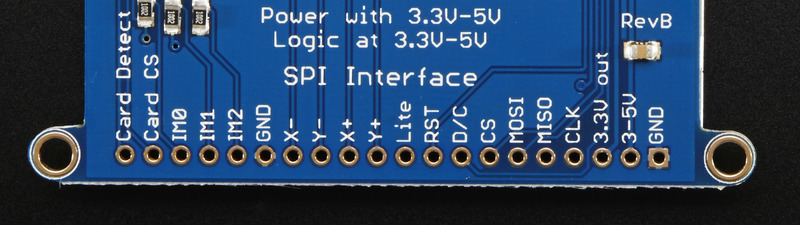
\includegraphics[width=0.8\linewidth]{images/HX8357_pinout.png}
    \caption{Pinout del Display HX8357}
    \label{fig:HX8357_pinout}
\end{figure}
\noindent Il display viene controllato mediante l'interfaccia/protocollo Serial Peripheral Interface (SPI) il quale richiede il collegamento dei seguenti pin:
\begin{itemize}
    \item alimentazioni: \texttt{VCC} ($3.3$V) e \texttt{GND}
    \item linee comuni: \texttt{MISO}, \texttt{MOSI} e \texttt{SCK}
    \item linea per il \textbf{chip select} (\texttt{CS})
\end{itemize}
Il Display HX8357 richiede il collegamento di un ulteriore pin \texttt{D/C} per la selezione della modalità data/command. Per i pin \texttt{MISO}, \texttt{MOSI} e \texttt{SCK} utilizziamo l'header \texttt{SPI} integrato nella scheda.